\documentclass[12pt]{article}
\usepackage{amsmath}
\usepackage{amssymb}
\usepackage{tikz}
\usepackage{multirow}

\usepackage{graphicx} 
\usepackage{float} 

\begin{document}

$Email: LE000288@umn.edu$\\

$ID:5674954$\\

$\textbf{Question 1}$\\

a)\\

Classifier 3: Decision Tree\\

Decision Tree would separate the data set based on some values using straight lines. For Figure1(A),it has two cuts, which makes the the two-dimensional data set with two target classes separate with specific x and y value.\\

b)\\

Classifier 1: Linear Support Vector Machine\\

Linear Support Vector Machine is a classifier looking for a separating hyperplane with the largest margin. For a two-dimensional data, it searches for a separating line. Since the classification boundary in Figure1(B) is a line, it means the classification boundary is linear.   The Linear Support Vector Machine has been used.\\

c)\\

Classifier 2: 1- Nearest Neighbor classifier\\

Nearest-neighbor classifiers can produce decision boundaries of arbitrary shapes. The classification boundary in Figure1(C) is irregular, thus we know it is 1-Nearest Neighbor classifier.



\newpage

$\textbf{Question 2}$\\

(a)\\

M2 would perform better.\\

For KNN, redundant attributes bias the proximity
measure towards certain attributes,resulting in improper estimates of distance.Hence, the presence of redundant attributes can make the performance of nearest neighbor classifiers worse.\\

(b)\\

M1 and M2 would be similar.\\

ANN can handle redundant attributes because weights are automatically learnt. Thus, redundant attributes receive similar weights and do not degrade the quality of the classifier. There is an exception that if the number of redundant attributes is large, the learning of the ANN model may suffer from overfitting, leading to poor generalization performance. But for this question, we only have one redundant attribute. It is safe to say that the two models would be similar.\\

\newpage

$\textbf{Question 3}$\\

(a) Decision Trees.\\

In this question, These attributes are appear to be of
varying relevance. Decision Trees can use measures such as the Gini index, gain ratio, to perform variable selection and allow irrelevant variables to be discarded.\\

Furthermore, the decision tree process is much like the process of a person making a decision. We could judge if we want to live near to Minneapolis and Saint Paul Downtown, live near to shopping malls,etc. But for SVM, it is hard to explain the hyperplane,hard-margin,soft-margin, Lagrange multipliers,etc. For KNN, it is also hard to interpret the cosine similarity, correlation , Euclidean distance,etc.\\

(b)\\

Decision Trees. \\

Decision Trees could handle the missing values in the training and test data easily by deciding which branch to follow if the value of a splitting node attribute is missing for a given test instance.Furthermore,  C4.5 decision tree classifier,CART algorithm and CHAID algorithm could help us handle the missing value in three different approaches.\\

For RIPPER, it is not well-suited for handling missing values in the training and test data because the position of rules in a rule set follows a certain ordering strategy. By using an ordered rule set, the presence of missing values can trigger the incorrect rule and result in incorrect class assignments.\\

(c)\\

RIPPER.\\

Since there are few houses that have high cost RIPPER chooses the majority class as its default class and learns the rules to detect instances from the minority class. So RIPPER is better for handling class imbalance because ordered rule sets it constructed. \\

Also, the attributes in this question appear to be of varying relevance, KNN’s performance can be adversely impacted by irrelevant attributes, as they can unduly influence the similarity function. So I prefer RIPPER to KNN.\\

\newpage

$\textbf{Question 4}$\\

(a)\\

K = 1\\

In this scenario, the blue pluses and the red circles do not mix with each other and do not have any noise. Furthermore, they have clear boundary. So we can use K = 1 to obtain the better performance. K = 5 and K = 50 are unnecessary and may cause some misclassification when the new data point shows in the middle because the red circles are more dense than the blue pluses.\\

(b)\\

K = 5\\

In this scenario, the blue pluses and the red circles separate with each other in most part. Only some sparse blue pluses show in the left side where most red circles located and only some sparse red circles show in the right side where most blue pluses located. To improve the generalization performance of the model, we cannot choose K = 1 in this scenario. Because K = 1 will let us misidentify the category of the data point. For example, if a new data point. Meanwhile, K = 50 is unnecessary and would cause misclassification when the new data point shows near the middle. In general, K = 5 would be the best one.


\newpage

$\textbf{Question 5}$\\

(a)\\

\begin{table}[]
\begin{tabular}{llll}
                              & \multicolumn{3}{l}{Predicted class}     \\
\multirow{3}{*}{Actual Class} &            & Class = a+    & Class = a- \\
                              & Class = a+ & 0.1(1000p)         & 0.1(1000(1-p))  \\
                              & Class = a- & 0.9(1000p) & 0.9(1000(1-p)) 
\end{tabular}
\end{table}


Expected precision for C0: \\

$100p/ 1000p = 0.1$\\

Recall for C0:\\

$100p/(100p+100-100p) = p$\\


(b)\\

F-measure for C0: \\

$\frac{200p}{200p+100-100p+900p}$\\

= $\frac{200p}{1000p+100}$\\

= $\frac{2p}{10p+1}$\\

(c)\\


F-measure for C0 = $\frac{2p}{10p+1}$\\

solving $\frac{2p}{10p+1} = 0.15$, p = 0.3\\

$\therefore$ When $0 <= p <= 0.3$, C1 is better. When $0.3 < p <= 1$, C0 is better\\


\newpage

$\textbf{Question 6}$\\

(a)\\

Dataset 1:\\

Precision = 0.8\\

Recall = 0.8\\

TPR = 0.8\\

FPR = 0.2\\

Dataset 2:\\

Precision = 0.44\\

Recall = 0.8\\

TPR = 0.8\\

FPR = 0.2\\

(b)\\

$\{TPR,FPR\}$\\

True positive rate (TPR) is defined as the fraction of positive test instances correctly predicted by the classifier.\\

False positive rate (FPR), which is defined as the fraction of negative test instances incorrectly predicted by the classifier.\\

Both evaluation are invariant to changes in the relative numbers of positives and negatives.\\

(c)\\

Accuracy: 0.8\\

To achieve better accuracy without even looking at the attributes of the data, we can predict all the data points to be negative, which means we will have 500 TN data points and 100 FN data points.\\

Accuracy = 500/600 = 0.833, thus the accuracy of this trivial classifier would be 0.833.\\

\newpage

$\textbf{Question 7}$\\

(a)\\

\begin{figure}[H] 
\centering 
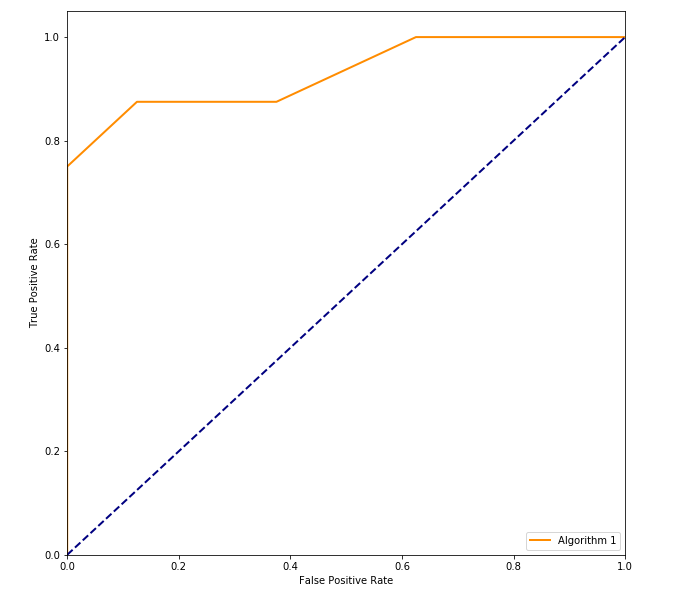
\includegraphics[width=0.7\textwidth]{algo1} 
\end{figure}

\begin{figure}[H] 
\centering 
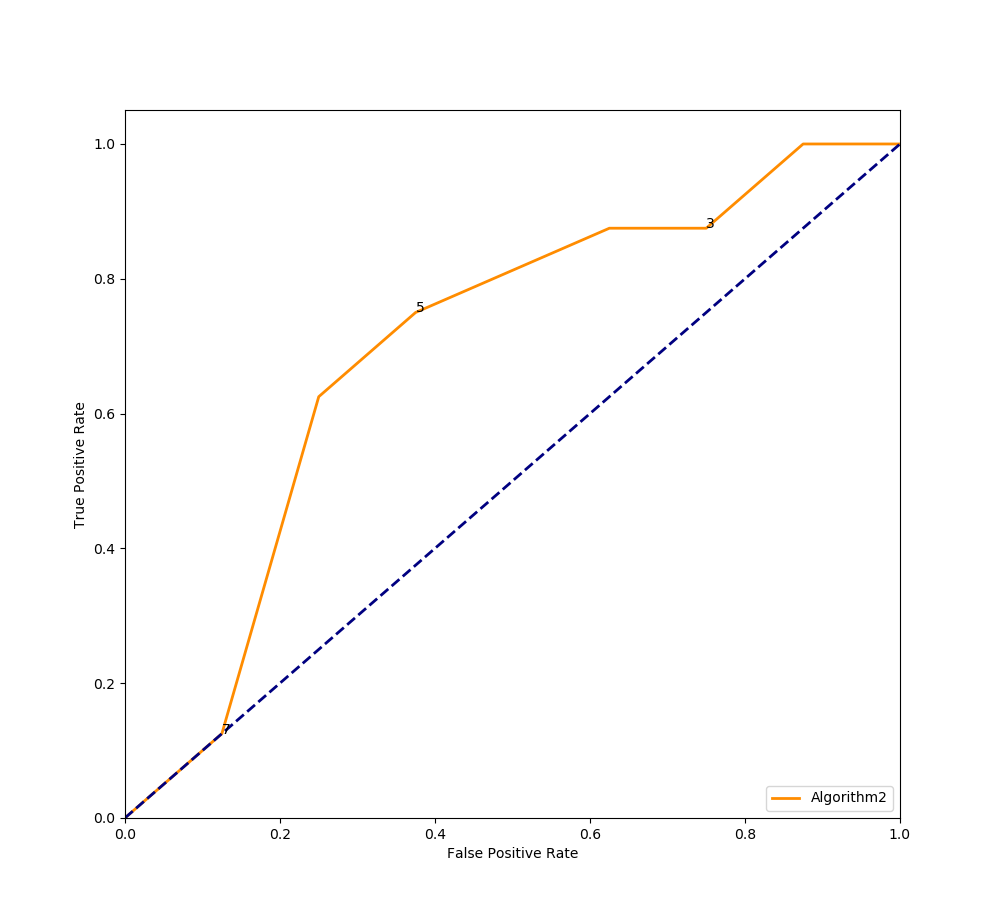
\includegraphics[width=0.7\textwidth]{algo2} 
\end{figure}

(b)\\

$\textbf{Thresholds 3:}$ \\

For data set 1:\\

$\because \frac{TP}{TP+FN} = 0.875$ and $\frac{FP}{FP+TN} = 0.75$\\

$\therefore TP = 7FN, FP = 3TN$\\

$\because TP + FN = 1000, FP + TN = 100$\\

$\therefore TP = 875, FN = 125, FP = 75, TN = 25$\\

expected precision = 0.921\\

recall = 0.875\\

TPR = 0.875\\

FPR =0.75\\

F-measure = 0.897\\

For data set 2:\\

$\because \frac{TP}{TP+FN} = 0.875$ and $\frac{FP}{FP+TN} = 0.75$\\

$\therefore TP = 7FN, FP = 3TN$\\

$\because TP + FN = 1000, FP + TN = 1000$\\

$\therefore TP = 875, FN = 125, FP = 750, TN = 250$\\

expected precision = 0.538\\

recall = 0.875\\

TPR = 0.875\\

FPR =0.75\\

F-measure = 0.667\\

$\textbf{Thresholds 5:}$ \\

For data set 1:\\

$\because \frac{TP}{TP+FN} = 0.75$ and $\frac{FP}{FP+TN} = 0.375$\\

$\therefore TP = 3FN, FP = 0.6TN$\\

$\because TP + FN = 1000, FP + TN = 100$\\

$\therefore TP = 750, FN = 250, FP = 37.5, TN = 62.5$\\

expected precision = 0.952\\

recall = 0.75\\

TPR = 0.75\\

FPR =0.375\\

F-measure = 0.839\\

For data set 2:\\

$\because \frac{TP}{TP+FN} = 0.75$ and $\frac{FP}{FP+TN} = 0.375$\\

$\therefore TP = 3FN, FP = 0.6TN$\\

$\because TP + FN = 1000, FP + TN = 1000$\\

$\therefore TP = 750, FN = 250, FP = 375, TN = 625$\\

expected precision = 0.667\\

recall = 0.75\\

TPR = 0.75\\

FPR =0.375\\

F-measure = 0.706\\

$\textbf{Thresholds 7:}$ \\

For data set 1:\\

$\because \frac{TP}{TP+FN} = 0.125$ and $\frac{FP}{FP+TN} = 0.125$\\

$\therefore TP = 0.143FN, FP = 0.143TN$\\

$\because TP + FN = 1000, FP + TN = 100$\\

$\therefore TP = 125, FN = 875, FP = 12.5, TN = 87.5$\\

expected precision = 0.91\\

recall = 0.125\\

TPR = 0.125\\

FPR =0.125\\

F-measure = 0.22\\

For data set 2:\\

$\because \frac{TP}{TP+FN} = 0.125$ and $\frac{FP}{FP+TN} = 0.125$\\

$\therefore TP = 0.143FN, FP = 0.143TN$\\

$\because TP + FN = 1000, FP + TN = 1000$\\

$\therefore TP = 125, FN = 875, FP = 125, TN = 875$\\

expected precision = 0.5\\

recall = 0.125\\

TPR = 0.125\\

FPR =0.125\\

F-measure = 0.2\\

$\textbf{For data set 1: threshold = 3}$ \\

$\textbf{For data set 2: threshold = 5}$ \\

(c)\\

By looking at the two ROC curves figures in part 1, algorithm 1 is better than algorithm 2 because the area under the ROC curve of algorithm 1 is larger than that of the algorithm 2 and the algorithm 1 has higher TPR than that of the algorithm 2 corresponding to any FPR.This means algorithm1 outperforms algorithm2 consistently.\\

\newpage

$\textbf{Question 8}$ \\

For cancer test, TP sample is the most important part, we are trying to choose the test which can show it has the higher accuracy on identifying TP. The second important evaluations are FN and FP, we are trying to choose the test with less FN and FP samples. \\

(a)\\

\begin{table}[]
\begin{tabular}{llll}
                              & \multicolumn{3}{l}{Predicted class  Question a}     \\
\multirow{3}{*}{Actual Class} &            & Class = +    & Class = - \\
                              & Class = + & 40         & 60  \\
                              & Class = - & 10 & 90 

\end{tabular}

\end{table}

Test 1 is better.\\

Compare test 1 to test 3, test 3 has better TPR, better precision and the F1-Score of test 3 is higher than those of test 1. But all these advantages are built on that test 1 has 1000 negative samples and test 3 only has 100 negative samples, which is imbalanced situation.\\

The more information I need: The FPR for test 1 stays same or not for different number of negative samples.\\

If the FPR of test 1 stays same.Then TPR becomes 0.4, FPR = 0.1, Precision becomes 0.8 and F1-Score becomes 0.444. We can say it is much better than test 3.\\

(b)\\

Test 1 is better.\\

T1 has higher TPR and higher F1-Score than those of T2. In general, T1 can identify the positive samples more accurate than that of the T2.Meanwhile, the FPR and Precision of these two samples are almost the same, which would not affect the result too much.\\

(c)\\

Test 4 is better.\\

T4 has higher TPR, higher F1-Score and higher precision than those of T1, which obviously shows that T4 can identify the positive samples more accurate than that of the T1 while the ability of identifying the negative sample stays the same.\\


\end{document}